\documentclass[class=book, crop=false, oneside, 12pt]{standalone}
\usepackage{standalone}
\usepackage{amsmath}
\usepackage{../../style}
\graphicspath{{./assets/images/}}

% arara: pdflatex: { synctex: yes, shell: yes }
% arara: latexmk: { clean: partial }
\begin{document}

\chapter{Dinamica dei sistemi di punti materiali}

\section{Sistemi di punti materiali, principio di azione e reazione}

Consideriamo un insieme \(n\) di punti materiali che interagiscono tra loro.\newline
La forza \(\overrightarrow{F}_i\) agente sull'\(i\)-esimo punto si può pensare come risultante delle \emph{forze esterne}
agenti sul punto \(\overrightarrow{F}_i^{(E)}\), e delle forze esercitate dagli altri \(n-1\) punti, forze interne al sistema \(\overrightarrow{F}_i^{(I)}\):
\begin{equation} \label{forze_interne_esterne}
    \overrightarrow{F}_i = \overrightarrow{F}_i^{(E)} + \overrightarrow{F}_i^{(I)}
\end{equation}
questa distinzione è utile ma, in ogni caso, non fa in modo che il moto sia diviso nelle due forze perché il moto di \(P_i\) dipende da \(\overrightarrow{F}_i\).

La distinzione tra forze interne ed esterne dipende da come viene definito il sistema di punti, che è arbitrario.

Alle forze interne si applica il principio di azione e reazione, indicato anche come terza legge di Newton. 
Se il punto \(i\)-esimo esercita sul punto \(j\)-esimo la forza \(\overrightarrow{F}_{i,j}\), il punto \(j\)-esimo reagisce esercitando sul punto \(i\)-esimo la forza \(\overrightarrow{F}_{j,i}\).
Si osserva che queste forze hanno la stessa direzione, verso opposto, stesso modulo e stessa retta di azione; esse possono essere attrattive o repulsive. 

\begin{figure}[h]
    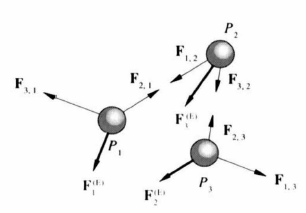
\includegraphics[scale=0.9]{forze_interne_azione_reazione}
    \centering
    \caption{}
\end{figure}

In generale la risultante \(\overrightarrow{F}_i^{(I)}\) delle forze interne agenti sull'\(i\)-esimo punto è diversa da zero, però la risultante di tutte le forze interne del sistema è nulla perché, in base al principio di azione e reazione, esse sono a due a due eguali ed opposte:
\begin{equation}
    \overrightarrow{R}^{(I)} = \sum_i \overrightarrow{F}_i^{(I)} = \sum_{i,j} \overrightarrow{F}_{i,j} = 0 
\end{equation}
con \(i  = 1,2,...,n\) , \(j = 1,2,...,n\) , \(i \neq j\).

\section{Centro di massa di un sistema di punti, Teorema del moto del centro di massa}

\subsection{Centro di massa}

Si definisce come centro di massa di un sistema di punti materiali il punto geometrico la cui posizione è individuata, nel sistema di riferimento considerato, dal raggio vettore:
\begin{equation}
    \overrightarrow{r}_{CM} = \frac{\sum_i {m_i \overrightarrow{r}_i}}{\sum_i m_i} = \frac{m_1 \overrightarrow{r}_1 + m_2 \overrightarrow{r}_2 + ... + m_n \overrightarrow{r}_n}{m_1 + m_2 + ... + m_n}
\end{equation}

Si noti che la posizione del centro di massa rispetto agli \(n\) punti materiali non dipende dal sistema di riferimento, mentre le sue coordinate invece variano a seconda del sistema prescelto.

Se gli \(n\) punti sono in movimento, di norma la posizione del centro di massa varia; sulla base della definizione calcoliamo la velocità del centro di massa:
\begin{equation}
    \overrightarrow{v}_{CM} = \frac{d \overrightarrow{r}_CM}{dt}
\end{equation}

Data \(M = \sum_i m_i\) la massa totale del sistema, vediamo che quindi che \(P\) coincide con la quantità di moto \(M \overrightarrow{v}_{CM}\) del centro di massa, considerato come un punto materiale che abbia la posizione \(\overrightarrow{r}_{CM}\), la velocità \(v_{CM}\) e massa pari alla massa totale \(M\) del sistema.

Analogamente possiamo ricavare l'accelerazione del centro di massa, derivando:
\begin{equation}
    \overrightarrow{a}_{CM} = \frac{d \overrightarrow{v}_{CM}}{dt} = \frac{\sum_i {m_i \frac{d \overrightarrow{v}_i}{dt}}}{\sum_i m_i} = \frac{\sum_i {m_i \overrightarrow{a}_i}}{\sum_i m_i} = \frac{\sum_i m_i \overrightarrow{a}_i}{M}
\end{equation}

Se il sistema di riferimento è inerziale
\begin{equation*}
    m_i \overrightarrow{a}_i = \overrightarrow{F}_i = \overrightarrow{F}_i^{(E)} + \overrightarrow{F}_i^{(I)}
\end{equation*}
secondo (\ref{forze_interne_esterne}) e sostituendo
\begin{equation}
    M \overrightarrow{a}_{C M}=\sum_i m_{i} \overrightarrow{a}_{i}=\sum_{i}\left(\overrightarrow{F}_{i}^{(E)}+\overrightarrow{F}_{i}^{(I)}\right)=\overrightarrow{R}^{(E)}+\overrightarrow{R}^{(I)}=\overrightarrow{R}^{(E)}
\end{equation}
dato che la risultante delle forze è nulla. 

\subsection{Teorema del moto del centro di massa}

La relazione
\begin{equation}
    \overrightarrow{R}^{(E)} = M \overrightarrow{a}_{C M}
\end{equation}
esprime il teorema del moto del centro di massa. 
Il centro di massa si muove come un punto materiale in cui sia concentrata tutta la massa del sistema e a cui sia applicata la risultante delle forze esterne.

Ho inoltre
\begin{equation}
    \overrightarrow{R}^{(E)} = M \overrightarrow{a}_{C M} = M \frac{d \overrightarrow{v}_{C M}}{dt} = \frac{d}{dt} \left( M \overrightarrow{v}_{C M}\right) = \frac{d \overrightarrow{P}}{dt}
\end{equation}
La risultante delle forze esterne è eguale alla derivata rispetto al tempo della quantità di moto totale del sistema. 

Il moto del centro di massa è determinato dunque solo dalle forze esterne. 
L'azione delle forze interne non può modificare lo stato di moto del centro di massa; invece il moto di ciascun punto dipende dall'azione delle forze esterne ed interne agenti su di esso.

\section{Conservazione della quantità di moto}

Se il sistema di punti considerato è isolato, cioè non soggetto a forze esterne, oppure l'azione delle forze esterne è tale che la loro risultante \(\overrightarrow{R}^{(E)}\) sia nulla, si ha:
\begin{equation}
    \overrightarrow{a}_{CM} = 0 \ , \ \overrightarrow{v}_{CM} = costante \ , \ \overrightarrow{P} = costante
\end{equation}

Quando la risultante delle forze esterne è nulla, la quantità di moto totale del sistema rimane costante nel tempo e il centro di massa si muove di moto rettilineo uniforme o resta in quiete. 
Tale risultato esprime il \emph{principio della conservazione della quantità di moto} per un sistema di punti materiali. 

La conservazione della quantità di moto può avvenire anche parzialmente, cioè essere riferita a una o due delle componenti. 
Per esempio se \(R_x^{(E)}\), allora \(P_x = costante\). 
Osserviamo poi che, pur verificandosi \(\overrightarrow{R}^{(E)}\), le quantità di moto dei vari punti \(m_i \overrightarrow{v}_i\) in generale variano nel tempo; resta costante solo la loro somma \(\sum_i m_i \overrightarrow{v}_i\).

\subsection{Esempio di due punti isolati}

Consideriamo ora due punti isolati, che possono quindi interagire solo tra loro: 
\begin{equation}
    \overrightarrow{P} = \overrightarrow{p}_1 + \overrightarrow{p}_2 = m_1 \overrightarrow{v}_1 + m_2 \overrightarrow{v}_2 = costante
\end{equation}
Derivando rispetto al tempo
\begin{equation*}
    \frac{d}{dt} \left(m_1 \overrightarrow{v}_1 + m_2 \overrightarrow{v}_2\right) = m_1 \overrightarrow{a}_1 + m_2 \overrightarrow{a}_2 = 0 
\end{equation*}
\begin{equation*}
    \implies \overrightarrow{F}_1 + \overrightarrow{F}_2 = 0 \ , \ \overrightarrow{F}_1 = - \overrightarrow{F}_2
\end{equation*}

Il principio di conservazione della quantità di moto per un sistema isolato di due punti ha come conseguenza che le forze che si esercitano tra i due punti sono eguali in modulo e di verso opposto.

Il risultato, però, non è completamente equivalente al principio di azione e reazione in quanto non implica che le due forze abbiano la stessa retta di azione.

\section{Osservazioni sulle proprietà del centro di massa}

La definizione introdotta di centro di massa è matematica, nel senso che non esiste il punto materiale centro di massa, ma la massa è distribuita nei singoli punti che si muovono sotto l'azione delle forze interne ed esterne. 
Tuttavia questo punto matematico gode di notevoli proprietà.

Per ora è stato dimostrato che, se si assume di concentrare in esso la massa del sistema, 
\begin{itemize}
    \item la sua quantità di moto è eguale a quella totale del sistema
    \item la sua accelerazione è determinata dalla risultante delle forze esterne agenti sul sistema
\end{itemize}

Il fatto che ad un certo istante \(\overrightarrow{v}_{CM}\) abbia un determinato valore significa solamente che il sistema in media si sta spostando in quella data direzione, anche se nessuna delle singole \(\overrightarrow{v}_i\) coincide con \(v_{CM}\).
Questo avviene analogamente anche per \(\overrightarrow{a}_{CM}\).

In effetti \(\overrightarrow{r}_{CM}, \overrightarrow{v}_{CM}\) e \(\overrightarrow{a}_{CM}\) sono le medie pesate sulle masse dei raggi vettori, velocità, accelerazioni dei singoli punti e pertanto forniscono informazioni di proprietà medie e non sul moto dei singoli punti. 

\section{Urti tra due punti materiali}

Quando due punti materiali vengono a contatto e interagiscono per un intervallo di tempo trascurabile rispetto al tempo di osservazione del sistema, si parla di urto tra i due punti.
Data la brevità del fenomeno si assume che durante l'interazione i punti non si muovano in modo apprezzabile.

Nell'urto si possono sviluppare forze molto intense che modificano la quantità di moto di ciascun punto.
Queste forze che, come avviene in un urto, agiscono per un tempo breve rispetto al tempo di osservazione, sono chiamate forze impulsive.

Osserviamo che le forze che si manifestano durante il processo d'urto sono forze interne al sistema costituito dai due punti materiali interagenti. 
In assenza di forze esterne si verifica pertanto durante l'urto la conservazione della quantità di moto totale.

Se indichiamo con \(\overrightarrow{v}_{1,in}\), \(\overrightarrow{v}_{2,in}\), le velocità nell'istante precedente all'urto dei due punti materiali, di masse \(m_1\) e \(m_2\), e con \(\overrightarrow{v}_{1,fin}\), \(\overrightarrow{v}_{2,fin}\), le corrispondenti velocità nell'istante successivo all'urto, la conservazione di \(\overrightarrow{P}\) si scrive:
\begin{equation}
    \overrightarrow{P}_{in} = m_1 \overrightarrow{v}_{1,in} + m_2 \overrightarrow{v}_{2,in} = m_1 \overrightarrow{v}_{1,fin} + m_2 \overrightarrow{v}_{2,fin} = \overrightarrow{P}_{fin}
\end{equation}
La quantità di moto del centro di massa rimane invariata nell'urto invece variano le quantità di moto di ciascun punto materiale per effetto dell'impulso della forza di interazione.
\begin{equation*}
    m_{1} \boldsymbol{v}_{1, fin}-m_{1} \boldsymbol{v}_{1, in}=\mathbf{I}_{2,1}=\int_{t_1}^{t_2} \mathbf{F}_{2,1} d t
\end{equation*}
\begin{equation*}
    m_{2} \boldsymbol{v}_{2, fin}-m_{2} \boldsymbol{v}_{2, in}=\mathbf{I}_{1,2}=\int_{t_1}^{t_2} \mathbf{F}_{1,2} d t
\end{equation*}
Ho naturalmente
\begin{equation*}
    \overrightarrow{F}_{1,2} = - \overrightarrow{F}_{2,1} \implies \overrightarrow{I}_{1,2} = - \overrightarrow{I}_{2,1}
\end{equation*}

\subsection{Forze esterne}

Possiamo conservare la quantità di moto totale anche in presenza di forze esterne se la durata dell'urto è sufficientemente piccola e le forze esterne non sono impulsive.
Infatti la variazione di quantità di moto totale del sistema dovuta alle forze esterne è
\begin{equation*}
    \Delta \overrightarrow{P} = \int_{t_1}^{t_2} \overrightarrow{F}^{(E)} dt = \overrightarrow{F}_m^{(E)} \tau
\end{equation*}
e se \(\tau\) è molto breve \(\Delta P\) risulta trascurabile.
Il ragionamento non sarebbe corretto se \(F^{(E)}\) fosse impulsiva nell'intervallo \(\tau\) quanto in tal caso il valore medio \(F_m^{(E)}\) potrebbe assumere valori notevoli.

Ricordiamo infine che a priori non è noto se le forze interne che si sviluppano nell'urto sono conservative e pertanto non si può assumere la conservazione dell'energia meccanica del sistema durante l'urto.

\section{Urto completamente anelastico}

L'urto si chiama completamente anelastico quando i due punti restano attaccati dopo l'urto formando un unico corpo puntiforme di massa \(m_1 + m_2\).
Se \(\overrightarrow{v}_1\) e \(\overrightarrow{v}_2\) sono le velocità dei due punti, nell'istante prima dell'urto e \(\overrightarrow{v}'\) la velocità comune immediatamente dopo l'urto.
Ottengo che:
\begin{equation*}
    m_1 \overrightarrow{v}_1 + m_2 \overrightarrow{v}_2 = \left( m_1 + m_2 \right) \overrightarrow{v}' = \left( m_1 + m_2 \right) \overrightarrow{v}_{CM}
\end{equation*} 
\begin{equation*}
    \overrightarrow{v}_{CM} = \frac{m_1 \overrightarrow{v}_1 + m_2 \overrightarrow{v}_2}{m_1 + m_2}
\end{equation*}
\(\overrightarrow{v}_{CM}\) rimane invariata nell'urto. Le variazioni di quantità di moto dei singoli punti sono \(m_1 \overrightarrow{v}_{CM} - m_1 \overrightarrow{v}_{1}\) e \(m_2 \overrightarrow{v}_{CM} - m_2 \overrightarrow{v}_{2}\) e sono uguali ed opposte.

L'energia cinetica prima dell'urto è:
\begin{equation*}
    E_{k,in} = \frac{1}{2} m_1 v_1^2 + \frac{1}{2} m_2 v_2^2 = E_k' + \frac{1}{2} \left( m_1 + m_2 \right) v_{CM}^2
\end{equation*}
quella finale per il Teorema di König diventa: % TODO Teorema di Konig è in 5.7 (lo spieghiamo?)
\begin{equation*}
    E_{k,fin} = \left( m_1 + m_2 \right) v_{CM}^2 < E_{k,in}
\end{equation*}

Nell'urto completamente anelastico viene assorbita l'energia \(E_k'\), cioè l'energia cinetica rispetto al centro di massa prima dell'urto. 
È infatti dopo l'urto che non c'è più moto rispetto al centro di massa, in cui i due punti vengono a coincidere. 
Nella realtà l'energia cinetica \(E_k'\) viene in parte utilizzata per la deformazione permanente dei due corpi. 

\section{Urto elastico}

Si definisce come urto elastico un urto durante il quale si conserva anche l'energia cinetica esterna.
Questo comporta che le forze interne, che si manifestano durante l'urto, siano conservative. 
I due corpi reali che si urtano subiscono, durante l'urto, delle deformazioni elastiche, riprendendo la configurazione iniziale subito dopo l'urto.
L'energia potenziale del sistema prima e dopo l'urto è la stessa e pertanto, se si conserva l'energia meccanica, deve conservarsi anche l'energia cinetica.

Valgono quindi le equazioni:
\begin{equation*}
    \overrightarrow{P}_{in} = \overrightarrow{P}_{fin} \ , \ E_{k,in} = E_{k,out}
\end{equation*}

Il caso più generale è tridimensionale e abbiamo sei incognite, le componenti delle velocità dei due punti dopo l'urto, ma solo quattro equazioni.
Anche nel caso di urto nel piano, abbiamo quattro incognite e tre equazioni. 
Quindi per risolvere un problema di urto elastico nel piano o nello spazio, oltre a conoscere le velocità prima dell'urto bisogna avere qualche altra informazione sulle velocità dopo l'urto.
Invece nel caso unidimensionale (due punti che si muovono prima e dopo l'urto elastico lungo la stessa direzione) abbiamo due equazioni di conservazione e due incognite (le velocità dei due punti dopo l'urto) e possiamo risolvere il problema.

Scriviamo dunque in quest'ultimo caso:
\begin{equation*}
    m_1 v_{1,in} + m_2 v_{2,in} = m_1 v_{1,fin} + m_2 v_{2,fin} = \left( m_1 + m_2 \right) v_{CM}
\end{equation*}
\begin{equation*}
    \frac{1}{2} m_1 v_{1,in}^2 + \frac{1}{2} m_2 v_{2,in}^2 = \frac{1}{2} m_1 v_{1,fin}^2 + \frac{1}{2} m_2 v_{2,fin}^2
\end{equation*}

Per determinare i valori di \(v_{1,fin}\) e \(v_{2,fin}\) in funzione di \(v_{1,in}\) e \(v_{2,in}\) è più comodo considerare l'urto anche nel sistema di riferimento del centro di massa, dove \(P' =0\) e quindi: 
\begin{equation*}
    m_1 v_{1,in}' = -m_2 v_{2,in}' \ , \  m_1 v_{1,fin}' = -m_2 v_{2,fin}'
\end{equation*}
\begin{equation*}
    \frac{1}{2} m_1 {v'}_{1,in}^2 + \frac{1}{2} m_2 {v'}_{2,in}^2 = \frac{1}{2} m_1 {v'}_{1,fin}^2 + \frac{1}{2} m_2 {v'}_{2,fin}^2
\end{equation*}
Da queste ottengo:
\begin{equation*}
    v_{1,fin}' = - v_{1,in}' \ , \ v_{2,fin}' = - v_{2,in}'
\end{equation*}
nel sistema del centro di massa la quantità di moto di ciascun punto resta la stessa in modulo, cambiando solo di verso. 

Tornando nel sistema inerziale da:
\begin{equation*}
    v_{1,in} = {v'}_{1,in} + v_{CM} \ , \ v_{2,in} = {v'}_{2,in} + v_{CM}
\end{equation*}
\begin{equation*}
    v_{1,fin} = {v'}_{1,fin} + v_{CM} \ , \ v_{2,fin} = {v'}_{2,fin} + v_{CM}
\end{equation*}
e da 
\begin{equation*}
    {v}_{CM} = \frac{m_1 {v}_1 + m_2 {v}_2}{m_1 + m_2}
\end{equation*}
Ottengo:
\begin{equation}
    v_{1,fin} = \frac{\left(m_1 - m_2\right)v_{1,in} + 2 m_2 v_{2,in} }{m_1 + m_2}
\end{equation}
\begin{equation}
    v_{2,fin} = \frac{2 m_1 v_{1,in} + \left(m_2 - m_1\right)v_{2,in} }{m_1 + m_2}
\end{equation}

\subsection{Esempi}
\begin{itemize}
    \item \(m_1 = m_2 = m : v_{1,fin} = v_{2,in} \ , \ v_{2,fin} = v_{1,in}\) \newline
    Si ottiene a seguito dell'urto uno scambio delle velocità. 

    \begin{figure}[h]
        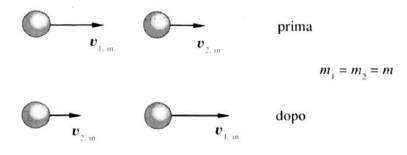
\includegraphics[scale=1]{urto_due_punti_materiali}
        \centering
    \end{figure}

    \item \(m_1 >> m_2 = m : v_{1,fin} \cong v_{1,in} \ , \ v_{2,fin} = 2 v_{1,in} - v_{2,in}\) \newline
    Nell'urto la velocità di \(m_1\) rimane praticamente la stessa

    \begin{figure}[h]
        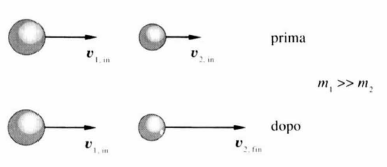
\includegraphics[scale=1]{urto_due_punti_materiali_diversi}
        \centering
    \end{figure}

    \item \(m_1 << m_2 = m \ e \ v_{2,in} = 0  \ : \ v_{1,fin} = - v_{1,in} \ , \ v_{2,fin} \cong 0 \) \newline
    In tale situazione \(m_1\) rimbalza all'indietro e \(m_2\) resta fermo. 
    Questo è un caso molto particolare, in cui possiamo verificare che si conserva l'energia cinetica, ma non la quantità di moto.
    Per esempio si tratta dell'urto di un punto contro un corpo massiccio, come una parete.
    Durante l'urto si sviluppano forze vincolari esterne di tipo impulsivo e quindi paragonabili a quelle interne. 
    Ciò non permette la conservazione della quantità di moto.

    \begin{figure}[h]
        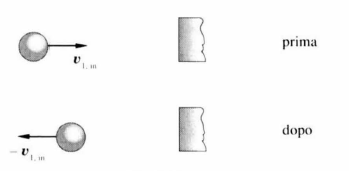
\includegraphics[scale=1]{urto_parete}
        \centering
    \end{figure}

    \item Urto obliquo contro una parete piana immobile liscia.\newline
    Anche questo è un caso particolare; è un urto bidimensionale, ma siccome uno dei due corpi è immobile è possibile risolvere il problema conoscendo la velocità prima dell'urto.
    Supponiamo che \(\overrightarrow{v}_{in}\) formi l'angolo \(\theta\) con la normale alla parete e abbia quindi le componenti \(v_{in} \sin \theta\) e \(v_{in} \cos \theta\). 
    Nella direzione parallela alla parete non c'è urto, si conserva la relativa quantità di moto e la componente della velocità vale ancora \(v_{in} \sin \theta\) dopo l'urto; 
    in direzione ortogonale abbiamo la situazione vista nel precedente caso e \(v_{in} \cos \theta\) diventa \(-v_{in} \cos \theta\). 
    Quindi \(v_{fin}\) è eguale in modulo a \(v_{in}\) e forma ancora l'angolo \(\theta\) con la normale alla parete. 

    \begin{figure}[h]
        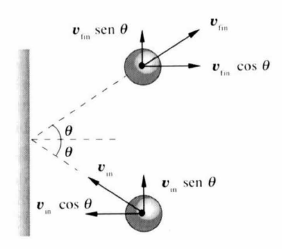
\includegraphics[scale=1]{urto_obliquo}
        \centering
    \end{figure}

\end{itemize}

\end{document}